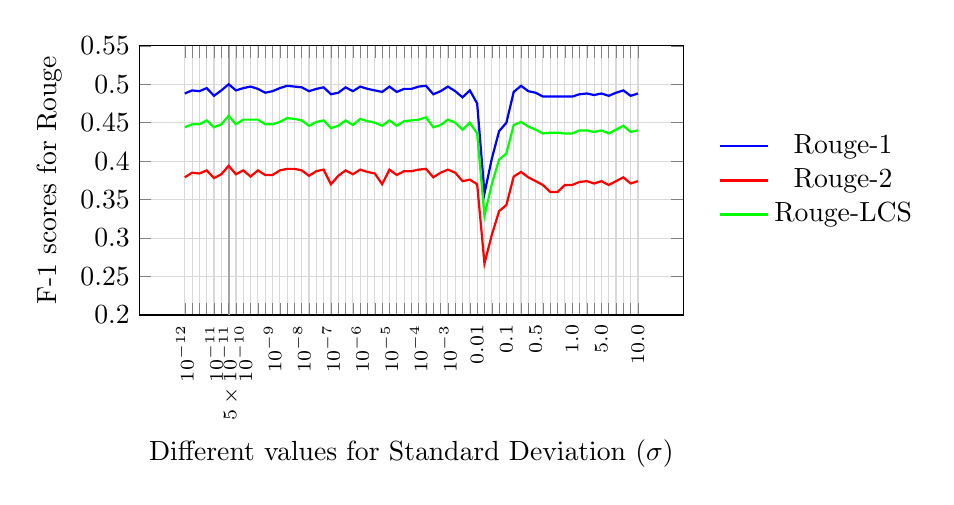
\begin{tikzpicture}
    \begin{axis}[
        width=.7\textwidth,
        height=5cm,
        xlabel={Different values for Standard Deviation ($\sigma$)},
        ylabel={F-1 scores for Rouge},
        ymin=0.2, ymax=0.55,
        xtick={1,2,...,63}, % Original 63 ticks
        xticklabels={ $10^{-12}$, , , , $10^{-11}$, ,$5\times10^{-11}$, , $10^{-10}$, , , , $10^{-9}$, , , , $10^{-8}$, , , ,
                     $10^{-7}$, , , , $10^{-6}$, , , , $10^{-5}$, , , , $10^{-4}$, , , ,
                     $10^{-3}$, , , , $0.01$, , , , $0.1$, , , , $0.5$, , , ,
                      , $1.0$, , , , $5.0$, , , , ,$10.0$}, % Show 1 in every 4 labels
        xticklabel style={rotate=90, anchor=east, font=\scriptsize}, % Rotate labels 90 degrees
        legend style={at={(1.05,0.5)}, anchor=west, draw=none}, % Move legend outside, remove border
        extra x ticks={7}, % Add extra tick for 7th position
        extra x tick style={grid=major, major grid style={gray!70, thick}}, % Style for the highlighted tic
        extra x tick labels={},
        grid=major,
        grid style={solid,gray!30},
        ytick={0.20, 0.25, 0.30, 0.35, 0.40, 0.45, 0.50, 0.55}, % Y-axis ticks
        cycle list name=color list
    ]

    % Dummy data for Column 1
    \addplot[color=blue, thick] coordinates {
        (1, 0.488)
        (2, 0.492)
        (3, 0.491)
        (4, 0.495)
        (5, 0.485)
        (6, 0.492)
        (7, 0.500)
        (8, 0.492)
        (9, 0.495)
        (10, 0.497)
        (11, 0.494)
        (12, 0.489)
        (13, 0.491)
        (14, 0.495)
        (15, 0.498)
        (16, 0.497)
        (17, 0.496)
        (18, 0.491)
        (19, 0.494)
        (20, 0.496)
        (21, 0.487)
        (22, 0.489)
        (23, 0.496)
        (24, 0.491)
        (25, 0.497)
        (26, 0.494)
        (27, 0.492)
        (28, 0.490)
        (29, 0.497)
        (30, 0.490)
        (31, 0.494)
        (32, 0.494)
        (33, 0.497)
        (34, 0.498)
        (35, 0.487)
        (36, 0.491)
        (37, 0.497)
        (38, 0.491)
        (39, 0.483)
        (40, 0.492)
        (41, 0.475)
        (42, 0.358)
        (43, 0.403)
        (44, 0.439)
        (45, 0.450)
        (46, 0.490)
        (47, 0.498)
        (48, 0.491)
        (49, 0.489)
        (50, 0.484)
        (51, 0.484)
        (52, 0.484)
        (53, 0.484)
        (54, 0.484)
        (55, 0.487)
        (56, 0.488)
        (57, 0.486)
        (58, 0.488)
        (59, 0.485)
        (60, 0.489)
        (61, 0.492)
        (62, 0.485)
        (63, 0.488)
    };
    \addlegendentry{Rouge-1}

    % Dummy data for Column 2
    \addplot[color=red, thick] coordinates {
        (1, 0.379)
        (2, 0.385)
        (3, 0.384)
        (4, 0.388)
        (5, 0.378)
        (6, 0.383)
        (7, 0.394)
        (8, 0.383)
        (9, 0.388)
        (10, 0.380)
        (11, 0.388)
        (12, 0.382)
        (13, 0.382)
        (14, 0.388)
        (15, 0.390)
        (16, 0.390)
        (17, 0.388)
        (18, 0.381)
        (19, 0.387)
        (20, 0.389)
        (21, 0.370)
        (22, 0.381)
        (23, 0.388)
        (24, 0.383)
        (25, 0.389)
        (26, 0.386)
        (27, 0.384)
        (28, 0.370)
        (29, 0.389)
        (30, 0.382)
        (31, 0.387)
        (32, 0.387)
        (33, 0.389)
        (34, 0.390)
        (35, 0.379)
        (36, 0.385)
        (37, 0.389)
        (38, 0.385)
        (39, 0.374)
        (40, 0.376)
        (41, 0.370)
        (42, 0.267)
        (43, 0.304)
        (44, 0.335)
        (45, 0.343)
        (46, 0.380)
        (47, 0.386)
        (48, 0.379)
        (49, 0.374)
        (50, 0.369)
        (51, 0.360)
        (52, 0.360)
        (53, 0.369)
        (54, 0.369)
        (55, 0.373)
        (56, 0.374)
        (57, 0.371)
        (58, 0.374)
        (59, 0.369)
        (60, 0.374)
        (61, 0.379)
        (62, 0.371)
        (63, 0.374)
    };
    \addlegendentry{Rouge-2}

    % Dummy data for Column 3
    \addplot[color=green, thick] coordinates {
        (1, 0.444)
        (2, 0.448)
        (3, 0.448)
        (4, 0.453)
        (5, 0.444)
        (6, 0.448)
        (7, 0.459)
        (8, 0.448)
        (9, 0.454)
        (10, 0.454)
        (11, 0.454)
        (12, 0.448)
        (13, 0.448)
        (14, 0.451)
        (15, 0.456)
        (16, 0.455)
        (17, 0.453)
        (18, 0.446)
        (19, 0.451)
        (20, 0.453)
        (21, 0.443)
        (22, 0.446)
        (23, 0.453)
        (24, 0.447)
        (25, 0.455)
        (26, 0.452)
        (27, 0.450)
        (28, 0.446)
        (29, 0.453)
        (30, 0.446)
        (31, 0.452)
        (32, 0.453)
        (33, 0.454)
        (34, 0.457)
        (35, 0.444)
        (36, 0.447)
        (37, 0.454)
        (38, 0.450)
        (39, 0.441)
        (40, 0.450)
        (41, 0.436)
        (42, 0.329)
        (43, 0.370)
        (44, 0.402)
        (45, 0.410)
        (46, 0.447)
        (47, 0.451)
        (48, 0.445)
        (49, 0.441)
        (50, 0.436)
        (51, 0.437)
        (52, 0.437)
        (53, 0.436)
        (54, 0.436)
        (55, 0.440)
        (56, 0.440)
        (57, 0.438)
        (58, 0.440)
        (59, 0.436)
        (60, 0.441)
        (61, 0.446)
        (62, 0.438)
        (63, 0.440)
    };
    \addlegendentry{Rouge-LCS}

    \end{axis}
\end{tikzpicture}